%%%%%%%%%%%%%%%%%%%%%%%%%%%%%%%%%%%%%%%%
%%%%% NATURE CLIMATE CHANGE FORMAT %%%%%
%%%%%%%%%%%%%%%%%%%%%%%%%%%%%%%%%%%%%%%%
%% Comment "% WPcomment" lines, uncomment "% NCCcomment" lines as well as the lines below, replace all citet/citep by cite

% \documentclass{nature}
% \usepackage{amsmath}
% \usepackage{amssymb}
% \usepackage{eurosym}
% % The following allows keeping figures within the text (otherwise nature.cls would ignore them)
% \usepackage{graphicx}
% \makeatletter
% \let\saved@includegraphics\includegraphics
% \AtBeginDocument{\let\includegraphics\saved@includegraphics}
% \renewenvironment*{figure}{\@float{figure}}{\end@float}
% \makeatother

% Nature guidelines (not NCC!)
% Sections can only be used in Articles.  Contributions should be organized in the sequence: title, text, methods, references, Supplementary Information line (if any), acknowledgements, interest declaration, corresponding author line, tables, figure legends.

% No subsubsection nor paragraph

% Spelling must be British English (Oxford English Dictionary)

%Each figure legend should begin with a brief title for the whole figure and continue with a short description of each panel and the symbols used. For contributions with methods sections, legends should not contain any details of methods, or exceed 100 words (fewer than 500 words in total for the whole paper). In contributions without methods sections, legends should be fewer than 300 words (800 words or fewer in total for the whole paper).

% Articles are restricted to 50 references,

% In addition, a cover letter needs to be written with the
% following:
% \begin{enumerate}
%  \item A 100 word or less summary indicating on scientific grounds
% why the paper should be considered for a wide-ranging journal like
% \textsl{Nature} instead of a more narrowly focussed journal.
%  \item A 100 word or less summary aimed at a non-scientific audience,
% written at the level of a national newspaper.  It may be used for
% \textsl{Nature}'s press release or other general publicity.
%  \item The cover letter should state clearly what is included as the
% submission, including number of figures, supporting manuscripts
% and any Supplementary Information (specifying number of items and
% format).
%  \item The cover letter should also state the number of
% words of text in the paper; the number of figures and parts of
% figures (for example, 4 figures, comprising 16 separate panels in
% total); a rough estimate of the desired final size of figures in
% terms of number of pages; and a full current postal address,
% telephone and fax numbers, and current e-mail address.
% \end{enumerate}

% See \textsl{Nature}'s website
% (\texttt{http://www.nature.com/nature/submit/gta/index.html}) for
% complete submission guidelines.

%%%%%%%%%%%%%%%%%%%%%%%%%%%%%%%%
%%%%% WORKING PAPER FORMAT %%%%%
%%%%%%%%%%%%%%%%%%%%%%%%%%%%%%%%
%% Comment "% NCCcomment" lines, uncomment "% WPcomment" lines as well as the lines below
\documentclass[12pt,english]{article}
\usepackage[utf8]{inputenc}
\usepackage{tgpagella} % Palatino text only
\usepackage{mathpazo}  % Palatino math & text
\usepackage[left=1.5in,right=1.5in,top=1.5in,bottom=1.5in]{geometry}
% \linespread{1.5}
\usepackage[super,comma,sort]{natbib} % WPcomment
% \usepackage[round,sort&compress]{natbib} % NCCcomment
\usepackage{url} % [hyphens]
\usepackage[hyperpageref]{backref} % back references biblio. Needs latexmk at compilation.
\usepackage[pagebackref]{hyperref}
% \usepackage{multibib} % incompatible with backref
\hypersetup{
  colorlinks=true, % breaklinks=true,
  urlcolor=purple,    % color of external links
  linkcolor=blue,  % color of toc, list of figs etc.
  citecolor=violet,   % color of links to bibliography
}
\usepackage{bm}
\usepackage{indentfirst}
\usepackage{tocbibind}
\setcitestyle{aysep={}} 
\usepackage{amsmath}
\usepackage{tcolorbox}
\usepackage{amssymb}
\usepackage{eurosym}
\usepackage{amsfonts}
\usepackage{enumerate}
\usepackage{babel}
\usepackage{graphicx}
\usepackage{caption}
\usepackage{supertabular}
\usepackage{tabularx}
\usepackage{float}
\usepackage{dsfont}
\usepackage{fancyvrb}
\usepackage{verbatim}
\usepackage{enumitem}
\usepackage{setspace}
\usepackage{comment}
\usepackage{subcaption}
\usepackage{tikz}
\usepackage{gensymb}
\usepackage{textcomp}

\usepackage{tabulary}
\usepackage{tabularx}
\usepackage{booktabs}
\usepackage{fullpage}
\usepackage{morefloats}
\usepackage{makecell}
\usepackage{lscape}
\usepackage{pdflscape}
\usepackage{longtable}
\usepackage{rotating}
\usepackage{fancyhdr}
\usepackage{tocloft}
\usepackage{titletoc}
\usepackage[export]{adjustbox}
\usepackage[anythingbreaks]{breakurl} % for links
\usepackage{multicol}
\newsavebox\ltmcbox % For net gain table over two columns
%\usepackage[nomarkers,figuresonly]{endfloat} % Figures at the end
%\usepackage[section,below]{placeins} % Floats placed in the section they appear in.
\renewcommand{\floatpagefraction}{.99}
\newenvironment{stretchpars}{\par\setlength{\parfillskip}{0pt}}{\par} % to justify a line

% % Getting landscape page and page number/footer on bottom of page (instead of to the left)
% \fancypagestyle{mylandscape}{
% \fancyhf{} %Clears the header/footer
% \fancyfoot{% Footer
% \makebox[\textwidth][r]{% Right
%   \rlap{\hspace{1.5cm}% Push out of margin by \footskip
%     \smash{% Remove vertical height
%       \raisebox{13.6cm}{% Raise vertically
%         \rotatebox{90}{\thepage}}}}}}% Rotate counter-clockwise
% \renewcommand{\headrulewidth}{0pt}% No header rule
% \renewcommand{\footrulewidth}{0pt}% No footer rule
% }

% \fancypagestyle{page_left}{%
% 	\renewcommand{\headrulewidth}{0pt}
%   \fancyhf{}
%   \fancyfoot[OC]{%
%       \begin{tikzpicture}[remember picture,overlay]
%           \node[xshift=1cm] (number) at (current page.west) {\thepage};
%       \end{tikzpicture}
%   }%
% }
% \renewcommand{\thesubfigure}{\Alph{subfigure}}

% \newcites{App}{Appendix References}

% \captionsetup[table]{skip=-10pt}
% \begin{document}

% \maketitle

% \clearpage
% % \startcontents
% % \printcontents{ }{1}{\section{\contentsname}}
% % \clearpage
% \section{Introduction\label{sec:intro}}

% % \clearpage
% \renewcommand{\bibsection}{\section{\refname}}
% \bibliographystyle{naturemag}
% \bibliography{global_tax_attitudes}
% % \stopcontents

% \end{document}


\title{Shortfall of Domestic Resources to Eradicate Extreme Poverty} 

\author{Adrien Fabre$^{1,2}$} % WPcomment
% \author{Adrien Fabre\footnote{CNRS, CIRED. E-mail: adrien.fabre@cnrs.fr.}
% I thank Michalis Moatsos for his help in using his data. I thank Thomas Goumont and Elise Thai for assistance. I declare that I also serve as president of Global Redistribution Advocates.} % NCCcomment TODO

\date{\today} % NCCcomment

\begin{document}

\sloppy
\maketitle

\begin{center}
{\textbf{\href{https://github.com/bixiou/domestic_poverty_eradication/raw/main/paper/poverty.pdf}{Link to most recent version}}}
\end{center}


% WPcomment
% \begin{affiliations}
% \item CNRS
% \item CIRED
% \end{affiliations}

% \begin{small} % NCCcomment
\begin{abstract}

\end{abstract}

% TODO!
\textbf{JEL codes:} 
\textbf{Keywords:} 

\tableofcontents

\onehalfspacing % NCCcomment

%\clearpage

\section{Introduction}% NCCcomment


\paragraph{Literature} 



\section{Results}
\subsection{Data}\label{subsec:data}
% => Why using PIP compared to alternatives (WIID adjusted to GDP; (GCIP stops in 2013; WID only covers 38 countries with post-tax data))? Most recent data and best estimation of poor's consumption.
% Not clear which is more accurate between survey and national accounts (Deaton 05), especially in low-income countries, as agricultural production is indirectly measured in national accounts. Also, in Africa, mean conso is similar between national accounts and surveys (Deaton 05). Also, WIID adjust to GDP PPP but I should adjust to national conso, not GDP. Martinez (22) shows that autocracies overestimate GDP growth by 35%. 
% Prydz et al. (22) argue that NAS are more accurate but show that the discrepancy between survey mean consumption and NAS HFCE is not that large: 22%, and 13.7% for low-income countries. HFCE is broader (and encompasses spending of non-profit entities like NGOs). => Also, if one scales up the conso distribution, one should also scale up the poverty line (as it is based on conso surveys): if one does that, poverty rates are on average the same, they change due to variation in survey/NAS discrepancies. 
% I can adjust to HFCE as robustness check https://data.worldbank.org/indicator/NE.CON.PRVT.PP.KD with the assumption that the extra money is held by the rich (>13$/day), 
The percentiles of each country's income (or consumption) are estimated by the Poverty and Inequality Platform (PIP) of the World Bank (ex-PovcalNet). This data is based on purchasing power parity (PPP) and given in constant 2017 \$. PIP aggregates the most recent household surveys (60\% of countries were surveyed between 2018 and 2021). 

In low-income countries (those of greatest interest to us), PIP provides data on the per capita \textit{consumption} (rather than income). Thereby, the data does not capture services procured by the government. Another potential concern with household surveys is that the aggregate (national) consumption they imply is generally lower than the one estimated in national accounts.\cite{deaton_measuring_2005,prydz_disparities_2022} This discrepancy comes from measurement errors on both sides: on the one hand, household surveys suffer from underreporting of top incomes and large expenditures; on the other hand, national accounts do not properly account for informal work %and auto-consumption, 
and tend to inflate agricultural output.\cite{aangrist_why_2021} 
Furthermore, autoritarian countries have been shown to produce inflated GDP statistics, except for countries below the GDP threshold of eligibility for preferential loans by the World Bank.\cite{martinez_how_2022} % international development association
While the ratio of Household Final Consumption Expenditures (HFCE) from national accounts is 44\% greater than the aggregate value from household surveys, the ``discrepancy ratio'' is largest for middle-income countries, and is only 12\% for low-income countries. 
Because household surveys are best suited to estimate consumption by the poorest, I use unadjusted PIP data in our baseline. 

As a robustness check, I also re-derive our main results after adjusting aggregate consumption by the discrepancy ratio (computed using World Bank data). In line with the literature,\cite{lakner_global_2013,anand_chapter_2015} I impute the extra consumption to the top percentile. I do not perform the rescaling on the 15\% of countries (like Burundi or the D.R.C.) with HFCE lower than its aggregate consumption from PIP, and I assume a discrepancy ratio of +12\% for the 20\% of countries lacking data on HFCE. 

As is common in this literature,\cite{karver_mdgs_2012,hellebrandt_future_2015,bicaba_can_2017} my baseline assumes ``balanced growth'', meaning that each percentile grows at the same rate between the country's survey year and 2030. 
I rescale incomes by the observed growth of GDP p.c. (in PPP) up to 2022 (using World Bank data) and by different methods for the 2022--2030 period. 
These methods include: extending the 2014--2019 growth trend (which excludes COVID years); extending the trend for growing countries and assuming no growth when GDP p.c. has contracted between 2014 and 2019; assuming a constant growth (of either 0\%, 3\%, 4.5\%, 6\%, or 7\%); using IMF forecasts\cite{imf_world_2023} (extended up to 2030 by replicating the 2026--2028 forecasted growth in 2028--2030); projecting future growth using an autoregressive quadratic model that predicts the 2011--2019 growth based on the 1991-2011 growth (then applied to 2022--2030 using the 2002--2022 growth). I deviate from this two-step procedure assess the original SDG goal, as I assume a constant growth of 7\% starting in 2015.



\subsection{The effect of balanced growth}

To estimate global poverty rates, the World Bank scales up the percentiles measured in household surveys by the country's GDP growth between the survey year and the year of interest. I project global poverty rates and poverty gaps in 2030 using the same assumption of balanced growth (i.e., constant inequality), for a range of growth scenarios (Table \ref{tab:poverty}). 

\begin{table}[h]

\caption[Global poverty (rates and gaps) in 2030 under different growth scenarios.]{\label{tab:poverty}Global poverty rates and poverty gaps in 2030 under different growth scenarios. Poverty rates are expressed in \% of world population and poverty gaps in \% of world GDP. Poverty lines are in PPP \$/day.}
\centering
\begin{tabular}[t]{lrrrrrrrr}
\toprule Growth scenario & \multicolumn{4}{c}{Poverty rate (\%)} & \multicolumn{4}{c}{Poverty gap (\% of GDP)} \\ 
 (Poverty line in \$/day)  & 2.15 & 3.65 & 6.85 & 18.15 & 2.15 & 3.65 & 6.85 & 18.15\\
\midrule
2022 Estimate & 7.3 & 21.1 & 44.4 & 72.2 & 0.26 & 1.36 & 7.01 & 42.96\\
Trend (2014--2019) & 6.2 & 14.4 & 34.5 & 66.2 & 0.21 & 0.87 & 4.29 & 30.64\\
Max(Trend, 0) & 6.3 & 14.2 & 34.3 & 66.4 & 0.19 & 0.81 & 4.16 & 30.25\\
Autoregressive projection & 6.2 & 15.2 & 36.8 & 65.5 & 0.17 & 0.84 & 4.64 & 32.02\\
3\% growth & 5.2 & 15.2 & 37.5 & 68.2 & 0.14 & 0.75 & 4.38 & 31.20\\
3\% unbalanced growth & 5.1 & 15.1 & 37.5 & 67.7 & 0.19 & 0.83 & 4.48 & 31.83\\
7\% growth & 2.2 & 8.5 & 25.5 & 59.5 & 0.05 & 0.29 & 1.93 & 18.07\\
7\% growth since 2016 & 1.1 & 3.1 & 15.3 & 51.3 & 0.01 & 0.08 & 0.74 & 10.15\\
\bottomrule
\end{tabular}
\end{table}

My estimates of 2022 global poverty rates closely align with the 2019 estimates from the World Bank: 9\% of the world population living with less than 2.15\$/day, 24\% below 3.65\$/day, and 47\% below 6.85\$/day. 
The poverty gap is the cost that separates people below the poverty line from that line. For example, if 10\% of the population earns 1.65\$/day and 90\% of the population earns more than 2.15\$/day, the poverty gap is $0.1 \cdot (2.15 - 1.65) = 0.05\$/\text{day}$. 
I estimate the extreme poverty gap at 0.25\% of the world GDP. This is a first approximation of what it would cost to lift everyone out of extreme poverty, defined with the \$2.15/day poverty line. 

Assuming that each country will continue to grow at the same rate as in the recent past, %grow over 2022--2030 at the same rate as over 2014--2019, %a balanced growth for 2022--2030 at the rate observed in the country over 2014--2019, 
I estimate that 6\% of the world population will live in extreme poverty in 2030. I find very similar estimates using a simple yet realistic model to predict a country's growth (an autoregressive projection based on its growth over the last 20 years). 
% With a balanced growth at a rate of 3\% in each country, extreme poverty would decline slightly more than in the realistic projections, at 5\%.
If each country grows by 3\% each year, extreme poverty would decline slightly more than in the realistic projections, at 5\%. 
Although steady growth reduces poverty, growth alone cannot achieve the first SDG: If the world grows by 7\% each year, the extreme poverty rate would still be 3\% in 2030. Even if the world had experienced a 7\% growth rate starting in 2015 (when the SDGs were adopted), extreme poverty would not be completely eliminated, at 1\% of the world population in 2030. 
As we cannot rely on growth alone to eliminate poverty, let us add domestic redistribution to the equation.

\subsection{Idealized redistributive policies}

Studying the arithmetics of inequality at the country level, I use the poverty gap to approximate the revenues required to eliminate poverty. 
In other words, I consider taxes on top incomes to finance a transfer to the poorest that would lift them at the poverty line. I consider two types of redistributive policies to close the poverty gap: (i) an ``antipoverty cap'' that would establish a ceiling on top incomes (and tax income at a 100\% rate above that threshold); (ii) an ``antipoverty tax'' that would raise a linear tax above a certain threshold. 

These policies are idealized and the estimate of revenue they generate should be seen as an upper bound of what could be achieved in practice, if they were implemented. First, I ignore any costs associated with raising a tax or transferring money, as if the lowest-income countries already had sufficient administrative resources. Second, any tax (and a fortiori a 100\% tax) reduces economic activity (real or declared). In this exercise, I abstract from tax distorsions and assume that the policies would not affect the taxable base.

If it were possible to expropriate top income individuals 
without reducing their economic activity, capping top incomes to finance an income floor would eliminate poverty at the lowest welfare cost. 
However, to protect private property and diminish the deterring effect on economic activity, governments would rather tax at a lower rate (than 100\%) and on a broader base (starting at a threshold deemed reasonable). 
Therefore, both the antipoverty cap and the antipoverty tax can be thought as rough but revealing approximations of the capacity to mobilize domestic resources.
% To fill the poverty gap at the least welfare cost, the cost should be borne by the wealthiest. Indeed, 
% If it were possible to expropriate top income individuals without reducing their economic activity, the welfare-maximizing transfer would consist of capping top incomes to finance an income floor. 
% Although in reality, an income cap would deter (declared) activity, %but abstracting from the distorsive aspect of the policy, 
% the income cap required to close the poverty gap can be used as a rough but revealing approximation of the capacity to mobilize national resources. 

With PIP data, we measure household consumption rather than income, meaning that we do not capture investment nor government spending. In other words, our idealized policies would leave productive investment and public services unaffected, an appropriate treatment given that these channels already contribute to growth and poverty reduction.

Unless otherwise stated, I use the scenario of balanced growth at a rate of 3\%. I choose this rate as a baseline as an upper bound of growth rates recently experienced in the lowest-income countries. Among the 8 countries with an average consumption below 3\$/day, growth was on average negative over 2014--2019 (or 2014--2022), and the highest growing country (Central African Republic) grew at a rate of 2.4\% per year. 

\subsection{Antipoverty caps}

I estimate the income cap that each country should impose to fill the extreme poverty gap with the exproriated income (Figure \ref{fig:antipoverty_cap}). 
In some countries like the D.R.C., even capping incomes at \$7/day would not suffice to raise revenues equal to the extreme poverty gap, despite a steady growth of 3\% per year between 2022 and 2030. 
In a very optimistic scenario of 7\% growth, the antipoverty cap would be \$14/day in the D.R.C. Also, note that there is no indication that the resources of this country are underestimated, as the aggregate consumption from household surveys is greater than HFCE from national accounts for the D.R.C. 
Besides, the D.R.C. is not the poorest country. 
In Madagascar, the average consumption would fall short of \$2.15/day in the baseline scenario, at \$2.02/day. This means that even with extreme redistribution, Madagascar does not have the domestic resources needed to eliminate extreme poverty by 2030. 
To give a last example of the shortfall of resources in the lowest-income countries, the antipoverty cap for Burundi in the scenario of 7\% growth would need to be as low as 8.60\$/day. 

\begin{figure}[h]
\caption{Income cap eradicating extreme poverty (in \$/day). In this idealized policy, all income above the cap is transferred to the extreme poor and lift them at \$2.15/day, assuming away distorsions, and after a yearly growth of 3\% over 2022--2030. %abstracting away from distorsions and implementation costs. Growth is 3\% over 2022--2030.
}\label{fig:antipoverty_cap}
\makebox[\textwidth][c]{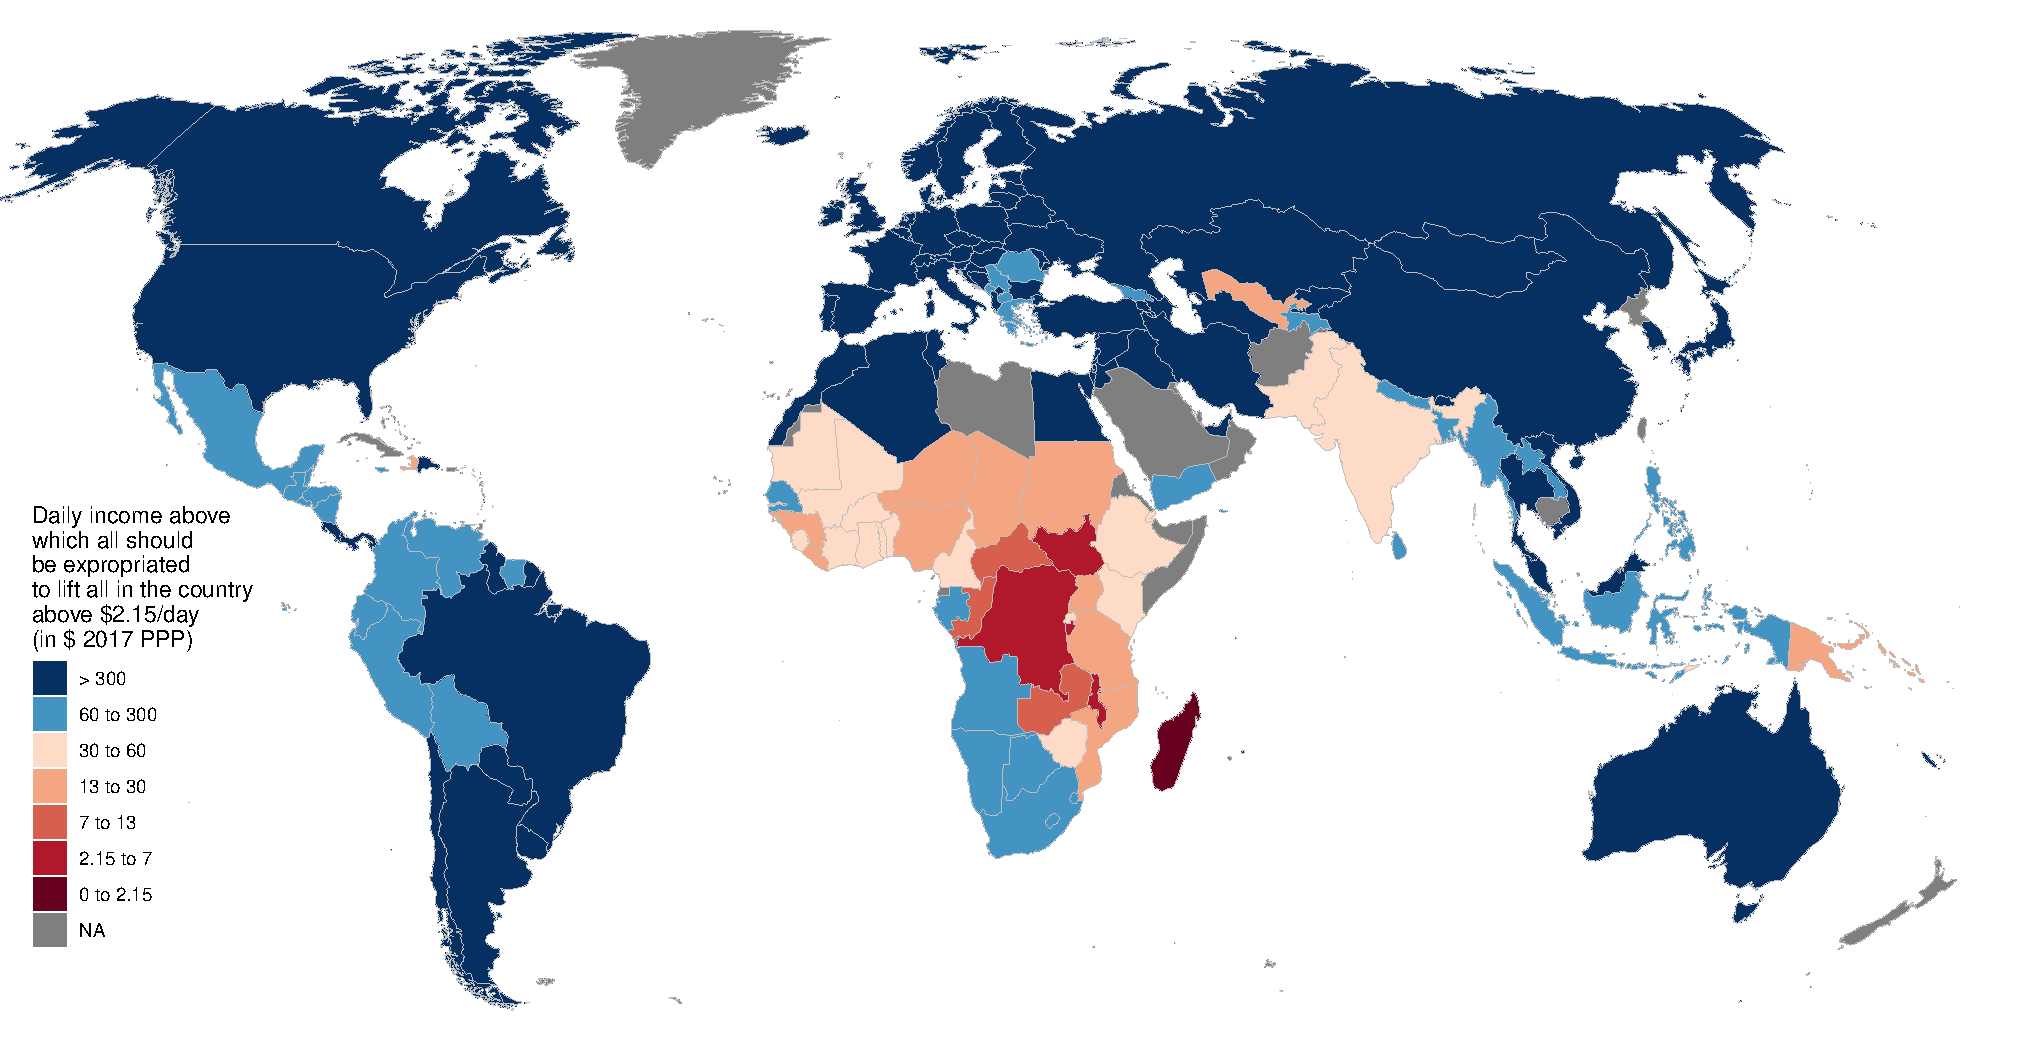
\includegraphics[width=\textwidth]
{../figures/y_expropriated_2_average.pdf}}
\end{figure}

\subsection{Antipoverty taxes}

Figure \ref{fig:antipoverty_tax_7} presents the (additional) tax rate above \$6.85/day required to generate enough revenues to close the domestic extreme poverty gap, in the baseline scenario of 
3\% growth. The threshold of \$6.85/day corresponds to a poverty line defined by the World Bank, which can be understood as the consumption level that can sustain a minimally decent life.\cite{hickel_is_2019,kikstra_decent_2021} In contrast, the extreme poverty line of \$2.15/day corresponds to the consumption per capita below which one is undernourished.\cite{allen_absolute_2017} 

\begin{figure}[h]
  \caption{Linear tax rate above \$6.85/day eradicating extreme poverty (in \%). In this idealized policy, all tax revenue is transferred to the extreme poor and lift them at \$2.15/day, assuming away distorsions, and after a yearly growth of 3\% over 2022--2030. 
  }\label{fig:antipoverty_tax_7}
  \makebox[\textwidth][c]{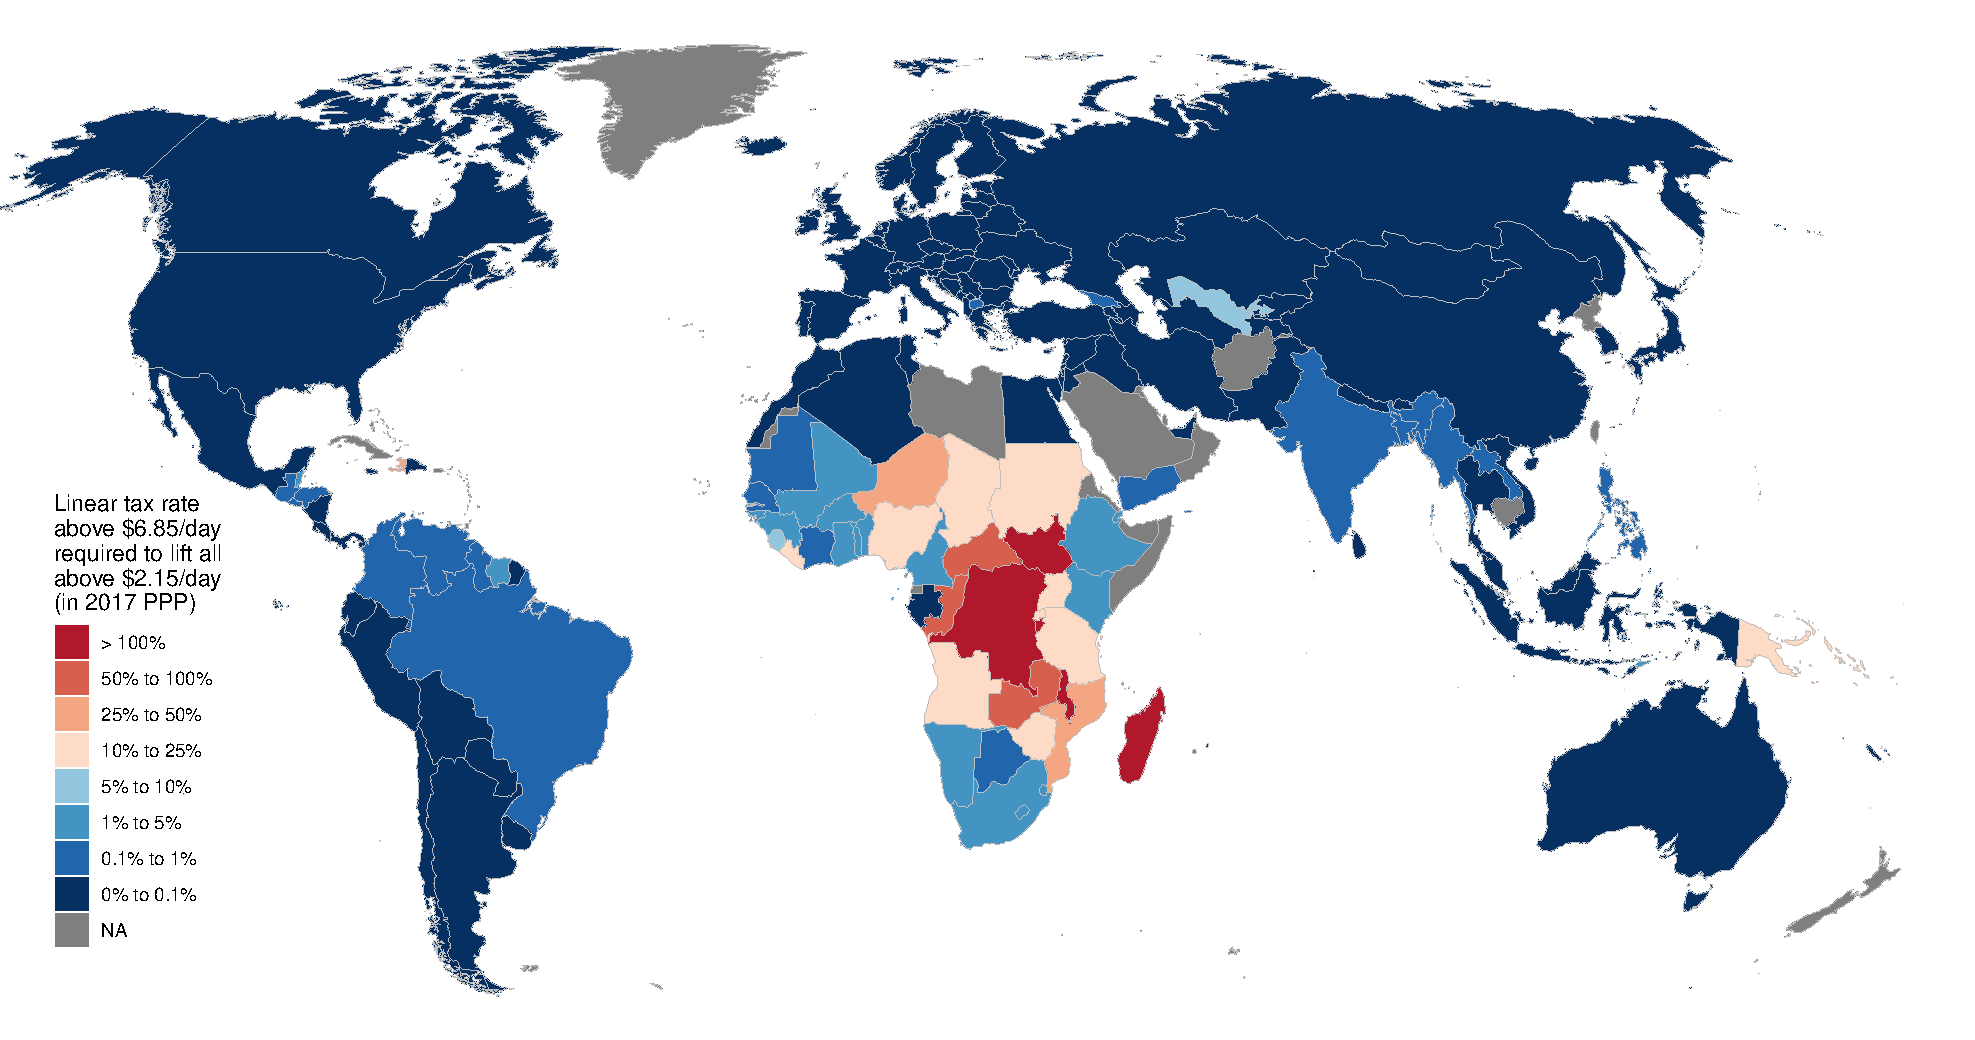
\includegraphics[width=\textwidth]
  {../figures/antipoverty_2_tax_7_average.pdf}}
\end{figure}

Consistently with the previous findings, taxing income at a 100\% rate above \$6.85/day would not generate enough revenues to eliminate extreme poverty in the five poorest countries. In Nigeria, closing the extreme poverty rate would require taxing the ``non-needy'' at a marginal rate of 20\%. On average over Sub-Saharan Africa, the anti-extreme-poverty tax would be 49\%, and 64\% in low-income countries (defined by the World Bank as countries with a GNI per capita below \$1,135 per year). Imposing such a large tax burden on any income above just \$6.85/day seems unrealistic. 

In most of the paper, we focus on the definition of extreme poverty employed in the first SDG. However, the \$2.15 threshold has been criticized for inaccurately measuring poverty. % TODO cite
First, this poverty line is too low to procure just a healthy diet, it is barely sufficient to satisfy one's caloric requirements. Second, the PPP adjustments applied to PIP data before computing the poverty rates are based on prices of the average consumption basket rather than on prices of subsistence goods.\cite{sullivan_capitalist_2023} Therefore, the cost of a subsistence diet varies across countries, e.g. at \$1.44 in Malawi vs. \$4.10 in Kenya (in 2011 PPP \$).\cite{moatsos_global_2016} Buidling on earlier work by Robert Allen,\cite{allen_absolute_2017} Michail Moatsos computes a country-specific poverty line by estimating the local price of the cheapest diet that meets caloric and protein requirements and of an allowance of  

Figure \ref{fig:antipoverty_tax_18} presents the anti-extreme-poverty tax on incomes above \$18.15/day, in a very optimistic scenario of 7\% growth. The threshold of \$18.15/day per person corresponds to the U.S. federal poverty line for a family of four and represents a more realistic threshold above which taxes could be increased in the Global South. The anti-extreme-poverty tax rates on the ``non-poor'' in this 7\% growth scenario are comparable to the rates on the non-needy in the baseline scenario. In India, the required tax rate would be \% in the scenario of 7\% growth, and \% if growth until 2030 replicates the 2014--2019 trend. % TODO
The contribution required of the Indian non-poor seems significant but not unreasonable. Therefore, India seems able to eliminate extreme poverty by 2030 with its domestic resources. The same thing cannot be said of Sub-Saharan Africa. %Therefore, lower-middle income countries like India seem able to eliminate extreme poverty by 2030 with its domestic resources. The same thing cannot be said of low-income countries, most of them in Sub-Saharan Africa. %

% By default, 6\% (7?) growth starting in 2023 
% - Tax rate to eradicate poverty: above 7, 18: Figure 2
% - Even worse when considering Moatsos' BCS line

\begin{figure}[h]
  \caption{Linear tax rate above \$18.15/day eradicating extreme poverty (in \%). In this idealized policy, all tax revenue is transferred to the extreme poor and lift them at \$2.15/day, assuming away distorsions, and after a yearly growth of 7\% over 2022--2030.
  }\label{fig:antipoverty_tax_18}
  \makebox[\textwidth][c]{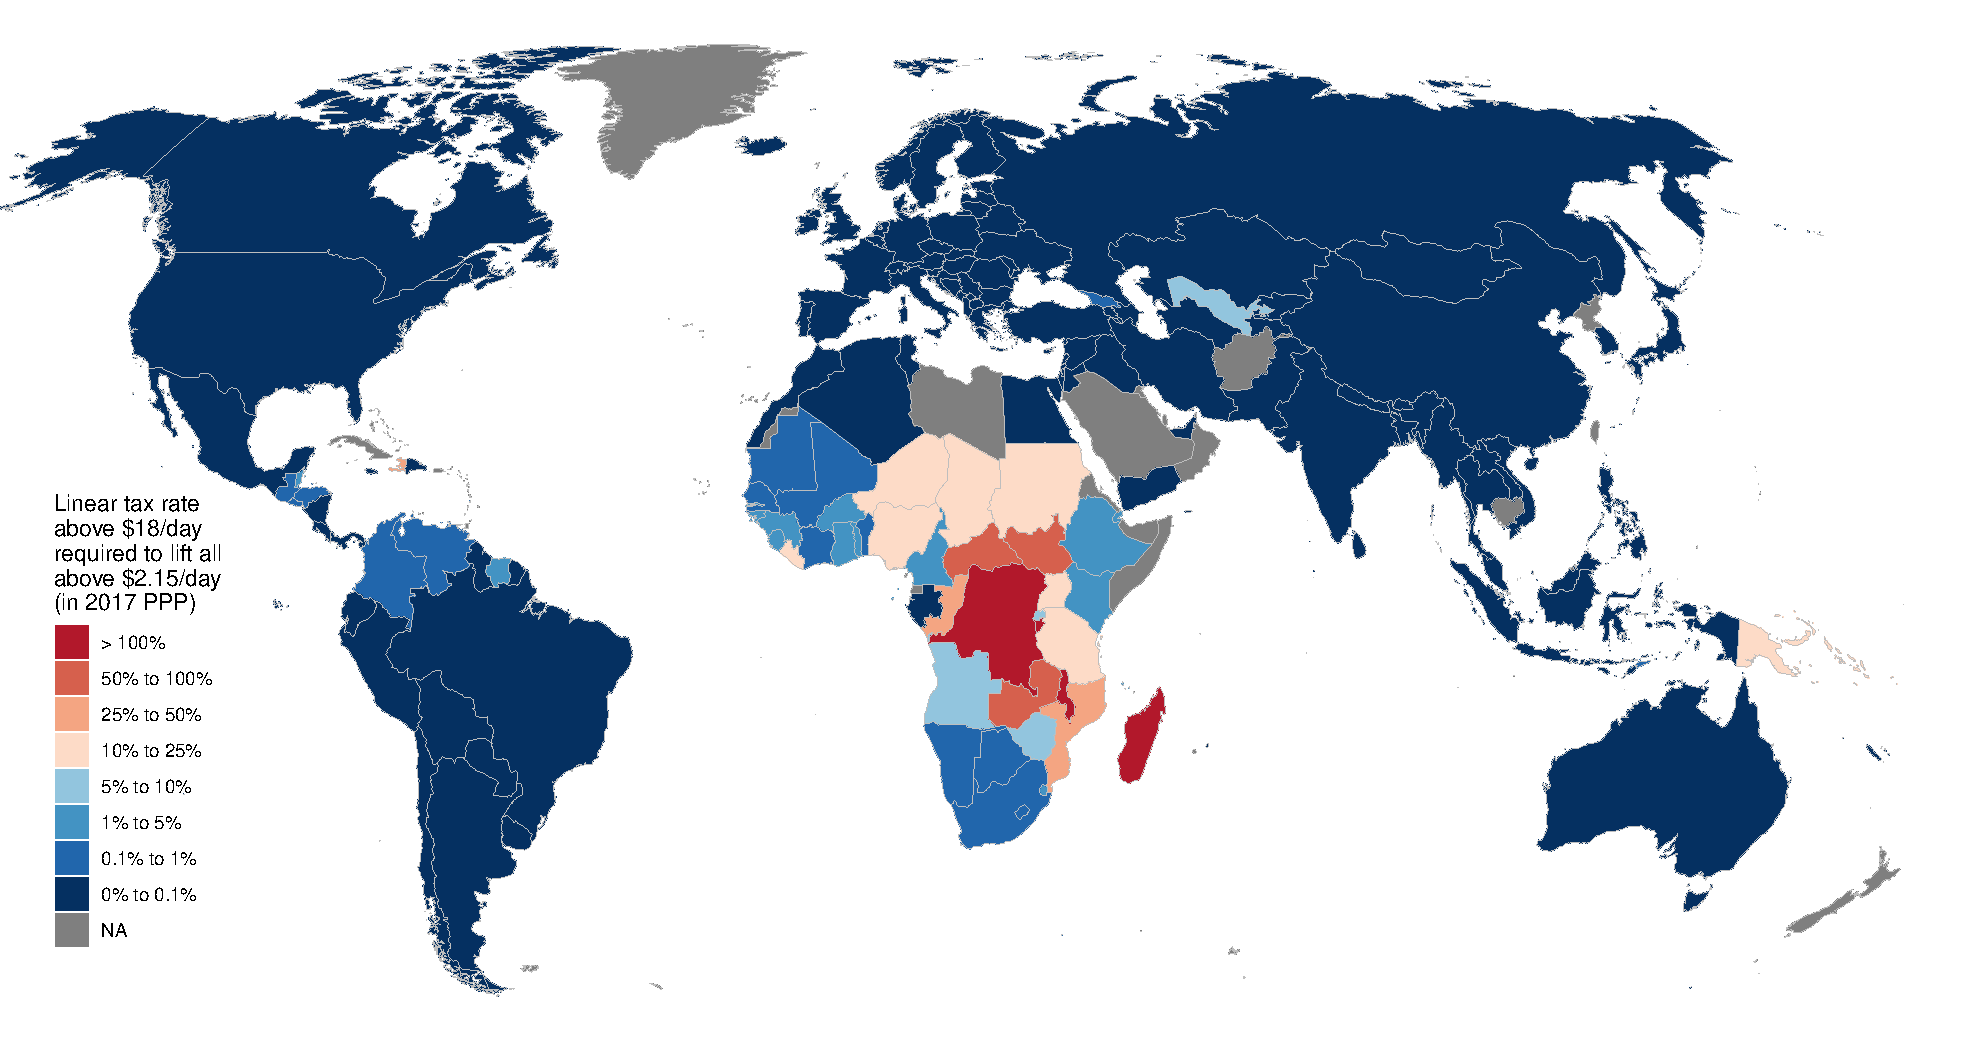
\includegraphics[width=\textwidth]
  {../figures/antipoverty_2_tax_18_very_optimistic.pdf}}
\end{figure}

\subsection{The credible potential of domestic redistribution}
% - Demogrant that can be funded with a given national tax: 5% above 7$  Figure 3
% - would have worked well if it had been 7\% since 2016



At least two of the SDGs spell out how the elimination of extreme poverty could be funded. % https://sdgs.un.org/2030agenda
First, the target 8.1 aims for ``at least 7 per cent gross domestic product growth per annum in the least developed countries''. % TODO: the previous tax would have been sufficient in the sdg8 scenario except in Madagascar, where a tax of 23% would have been required. In other words, a sustained high growth would have permitted the least developed countries to eliminate extreme poverty through the mobilization of their domestic resources. However, high growth has never materialized in these countries. 
Second, the target 17.2 calls for ``Developed countries to implement fully their official development assistance commitments, including the commitment by many developed countries to achieve the target of 0.7 per cent of ODA/GNI to developing countries and 0.15 to 0.20 per cent of ODA/GNI to least developed countries'' (LDCs). Foreign aid falls short of both the overall target (at 0.36\% of developed countries' GNI) and the LDCs' target (at 0.06\%). Although European countries taken together respect their commitment, the other do not. In particular, the U.S. only allocates 0.22\% of its GNI to foreign aid.\cite{oecd_oda_2023} The global extreme poverty gap (0.17\% of global real GDP) is a bit lower than the shortfall of foreign aid relative to the target (0.2\% of global nominal GDP), suggesting that extreme poverty could be eradicated if developed countries respected their commitment. % OECD (high-income) countries represent 59% (61%) of the world nominal GDP, so shortfall of aid is 0.34*0.59=0.2% of global GDP in nominal. https://data.worldbank.org/indicator/NY.GDP.MKTP.CD
% TODO? To meet the broader SDGs and ``end poverty in all its forms'', the 0.7\% target would not suffice and global redistribution would need to be significantly increased. 

\subsection{The potential of global redistribution}
% - One example of global redistribution (incl. largest recipients/contributors)
% - Inequality indicators BAU / national / global redistr: Table 2


\section{Discussion} 

% \begin{methods}  % WPcomment
  \begin{small} % NCCcomment
%Put methods in here.  If you are going to subsection it, use \subsection commands.  Methods section should be less than 800 words and if it is less than 200 words, it can be incorporated into the main text.
\section*{\normalsize Methods}\label{sec:methods} % NCCcomment
\addcontentsline{toc}{section}{\nameref{sec:methods}}
% \subsection*{\small Data quality.} % WPcomment % TODO attrition analysis
\paragraph{\small Data quality.} % NCCcomment


\section*{\normalsize Data and code availability}

All data and code of as well as figures of the paper are available on \href{https://github.com/bixiou/domestic_poverty_eradication}{github.com/bixiou/domestic\_poverty\_eradication}. 

% \end{methods} % WPcomment
\end{small}  % NCCcomment

% \bibliographystyle{naturemag_noURL} % nature class works only with style naturemag or naturemag_noURL, and naturemag bugs if there are certain URLs (like .pdf). Also, nature class only works with \cite, not \citet or \citep.  % WPcomment
\renewcommand{\url}[1]{\href{#1}{Link}} % NCCcomment
\bibliographystyle{plainnaturl_clean} % NCCcomment
\bibliography{poverty}

\appendix % NCCcomment
\renewcommand{\thetable}{A\arabic{table}}
\renewcommand{\thefigure}{A\arabic{figure}}
\setcounter{figure}{0}
\setcounter{table}{0}

% \input{app} 

\clearpage
\listoftables
\listoffigures
% WPcomment
%% Here is the endmatter stuff: Supplementary Info, etc.
%% Use \item's to separate, default label is "Acknowledgements"
% \begin{addendum} % 177 words
%  \item I are grateful 
%  \item[Competing Interests] The authors declare that they have no
% competing interests.
% \item[JEL codes] 
% \item[Keywords] 
%  \item[Correspondence] Correspondence and requests for materials
% should be addressed to Adrien Fabre~(email: fabre.adri1@gmail.com).
% \end{addendum}


\end{document}
